\documentclass[xetex,table]{beamer}

\usepackage[autostyle]{csquotes}
\usepackage{hyperref}
\usepackage{color}
\usepackage{setspace}
\usepackage{listings}
\usepackage{minted}

\usetheme{metropolis}

\usemintedstyle{perldoc}

\title{Build Automation:\\Introduzione a Make, Autotools e CMake}
\author{Luca Ceresoli\\
  \href{mailto:luca@lucaceresoli.net}{luca@lucaceresoli.net}\\
  \url{http://lucaceresoli.net}
}
\date{Linux Day 2017}

\begin{document}

\maketitle

\section{Introduzione}

\begin{frame}{Processo di build}
  \begin{center}
    \includegraphics[width=0.7\textwidth]{images/c-example.pdf}

    \pause
    \vspace{0.1\textheight}
    \texttt{gcc -o hello hello.c utils.c}
  \end{center}
\end{frame}

\begin{frame}{Processo di build}
  \begin{flushright}
    \includegraphics[width=0.33\textwidth]{images/c-example.pdf}
  \end{flushright}

  Processo di build:
  \begin{itemize}
  \item Input: il lavoro di un umano
  \item Output: un programma, una libreria, un documento, \dots
  \end{itemize}

  Esempi:
  \begin{itemize}
  \item Codice C / C++ \textrightarrow{} un eseguibile o una libreria
  \item File di testo \textrightarrow{} Un documento PDF
  \end{itemize}
\end{frame}

\begin{frame}{Dove andrà il tuo software domani?}
  \begin{itemize}
  \item Continuous integration / continuous delivery
    \begin{itemize}
    \item Jenkins, Travis CI...
    \item Server locale o ``cloud''
    \end{itemize}
    \pause
  \item Distribuzioni: dpkg, rpm...
    \pause
  \item Sistemi embedded
    \begin{itemize}
    \item Buildroot
    \item Openembedded
    \item OpenWRT
    \end{itemize}
    \pause
  \item Windows, MacOS, Android, iOS
  \end{itemize}
\end{frame}

\begin{frame}{Come vuoi compilare il tuo software?}
  \begin{itemize}
  \item Debug / Release
  \item \texttt{-Wall -Werror}
  \item Librerie: shared / static
  \item \dots
  \end{itemize}
\end{frame}

\begin{frame}{Build automation: necessità}
  \begin{itemize}
  \item Da riga di comando
  \item Deve funzionare in ambienti diversi
  \item Non deve avere {\em policy} hard-coded
  \end{itemize}
\end{frame}

\section{Shell script}

\definecolor{codebackground}{rgb}{0.96,0.96,0.75}

\begin{frame}[fragile]{Shell script semplice}
  \begin{center}
  \includegraphics[height=0.4\textheight]{images/shell.pdf}
  \end{center}

  \texttt{build.sh}:

  \inputminted[bgcolor=codebackground,frame=single]{shell}{examples/1-shell-1/build.sh}
\end{frame}

\begin{frame}{Shell script semplice}
  \begin{itemize}
  \item[\checkmark] Funziona per casi molto semplici
  \item[$\times$]   Ricompila tutto ogni volta (se ci sono 100 file sorgente?)
  \end{itemize}
\end{frame}

\begin{frame}{File oggetto intermedi}
  \center\includegraphics[height=0.5\textheight]{images/depend-graph.pdf}
\end{frame}

\begin{frame}[fragile]{File oggetto intermedi}
  \small\inputminted[bgcolor=codebackground,frame=single]{shell}{examples/1-shell-2/build.sh}
\end{frame}

\begin{frame}{File oggetto intermedi}
  \begin{itemize}
  \item[\checkmark] Più efficiente
  \item[$\times$]   Scomodo da scrivere e mantenere
  \item[$\times$]   Non sfrutta CPU multi core
  \end{itemize}
\end{frame}

\section{Make}

\begin{frame}{Make}
  \center\includegraphics[width=0.8\textwidth]{images/makefile.pdf}
\end{frame}

\begin{frame}{Makefile}
  \texttt{Makefile} contiene {\em regole}:

  \inputminted[bgcolor=codebackground,frame=single]{makefile}{examples/2-make-1/Makefile}
\end{frame}

\begin{frame}[fragile]{Regole}
  \begin{minted}[autogobble]{makefile}
    hello: hello.o utils.o
            gcc -o hello hello.o utils.o
  \end{minted}

  \begin{itemize}
  \item \texttt{hello} = target
  \item \texttt{hello.o utils.o} = dipendenze
  \item \texttt{gcc \dots} = comandi
  \end{itemize}
\end{frame}

\begin{frame}{Grafo delle dipendenze}
  \center\includegraphics[height=0.4\textheight]{images/depend-graph.pdf}
\end{frame}

\begin{frame}[fragile]{Uso di Make}
  \begin{minted}[autogobble]{shell-session}
    $ ls -tr
    utils.h  utils.c  hello.c  Makefile
    $ make
    gcc -c hello.c
    gcc -c utils.c
    gcc -o hello hello.o utils.o
    $ ls -tr
    utils.h  utils.c  hello.c  Makefile  utils.o  hello.o  hello
    $ touch utils.c
    $ make
    gcc -c utils.c
    gcc -o hello hello.o utils.o
    $
  \end{minted}
\end{frame}

\begin{frame}[fragile]{Altre regole utili}
  \begin{minted}[autogobble]{makefile}
    install:
        install -m 755 hello /usr/bin/

    clean:
        rm -f hello hello.o utils.o

    dist:
        tar czf hello.tar.gz utils.h utils.c hello.c Makefile
  \end{minted}
\end{frame}

\begin{frame}{Alcuni vantaggi di Make}
  \begin{itemize}
  \item Scrittura delle regole
    \begin{itemize}
    \item Wildcard (\texttt{\%.o: \%.c})
    \item Implicit rules: varie regole predefinite (C, C++, \dots)
    \item \dots
    \end{itemize}
  \item Utilizzo
    \begin{itemize}
    \item Build in parallelo (\texttt{make -j<N>})
    \item Build di un target specifico (\texttt{make utils.o})
    \end{itemize}
  \end{itemize}
\end{frame}

\begin{frame}{Cosa manca a Make}
  \begin{itemize}
  \item Ricerca di librerie
  \item Prefix (\texttt{/usr}, \texttt{/usr/bin}, \dots)
  \item Diverted installation (\texttt{DESTDIR})
  \item Out of tree build
  \item Cross-compilazione (possibile ma scomoda)
  \end{itemize}
\end{frame}

\section{Autotools}

\begin{frame}[fragile]
  \begin{center}
  \begin{verbatim}
    ./configure
    make
    sudo make install
  \end{verbatim}
  \end{center}
\end{frame}

\begin{frame}{Autotools: schema semplificato}
  \center\includegraphics[height=0.7\textheight]{images/autotools.pdf}
\end{frame}

\begin{frame}[fragile]{Autoconf}
  \begin{columns}
    \column{0.7\textwidth}
    \texttt{configure.ac}
    \inputminted[bgcolor=codebackground,frame=single]{shell}{examples/3-autotools-1/configure.ac}

    \begin{itemize}
    \item È uno script di shell
    \item Con l'aggiunta di macro \texttt{m4}
    \end{itemize}

    \column{0.3\textwidth}
    \includegraphics[width=\textwidth]{images/autotools-autoconf.pdf}
  \end{columns}
\end{frame}

\begin{frame}{Autoconf}
  \small

  \begin{columns}
    \column{0.7\textwidth}
    \texttt{configure.ac}
    \inputminted[bgcolor=codebackground,frame=single]{shell}{examples/3-autotools-2/configure.ac}

    \column{0.3\textwidth}
    \includegraphics[width=\textwidth]{images/autotools-config-files.pdf}
  \end{columns}

  \texttt{Makefile.in}
  \inputminted[bgcolor=codebackground,frame=single]{makefile}{examples/3-autotools-2/Makefile.in}
\end{frame}

\begin{frame}{Automake}
  \begin{flushright}
    \includegraphics[width=0.3\textwidth]{images/autotools-automake.pdf}
  \end{flushright}

  \texttt{Makefile.am}
  \inputminted[bgcolor=codebackground,frame=single]{makefile}{examples/3-autotools-3/Makefile.am}

  \begin{itemize}
  \item È un normale Makefile
  \item Con l'aggiunta di costrutti di \texttt{automake}
  \end{itemize}
\end{frame}

\begin{frame}[fragile]{Automake: PSV e PLV}
  \texttt{Makefile.am} si compone di:

  \begin{itemize}
  \item \mintinline{makefile}{bin_PROGRAMS = hello}
    \begin{itemize}
    \item Product List Variable (PLV)
    \item Elenca i {\em prodotti} da generare
    \end{itemize}
  \end{itemize}

  \begin{itemize}
  \item \mintinline{makefile}{hello_SOURCES = hello.c utils.c utils.h}
    \begin{itemize}
    \item Product Source Variable (PSV)
    \item Elenca i {\em sorgenti} necessari per generare un prodotto
    \end{itemize}
  \end{itemize}

\end{frame}

\begin{frame}{Autotools}
  \center\includegraphics[height=0.7\textheight]{images/autotools.pdf}
\end{frame}

\begin{frame}{Autotools: vantaggi}
  \begin{itemize}

  \item Usato da moltissimi software
  \item Compatibilità con ogni sistema UNIX-like
  \item Moltissime macro già pronte
  \item Usano shell e Make
  \item Generano \texttt{Makefile}:
    \begin{itemize}
    \item Conformi agli standard UNIX
    \item Completi (\texttt{make install},
    \texttt{make clean},
    \texttt{make dist}, \dots)
    \end{itemize}

  \item Vedi slide ``Cosa manca a Make'':
    \begin{itemize}
    \item Ricerca di librerie
    \item Prefix (\texttt{--prefix=/usr})
    \item Diverted installation (\texttt{DESTDIR})
    \item Out of tree build
    \item Cross-compilazione con strumenti standard
    \end{itemize}

  \end{itemize}
\end{frame}

\begin{frame}{Autotools: svantaggi}
  \begin{itemize}
  \item Praticamente inutilizzabili su sistemi non UNIX-like
  \item Usano shell e Make
  \item Complesso da imparare inizialmente
    \begin{itemize}
    \item È facile scrivere codice ``sbagliato'' se non è chiaro il
      come funzionano
    \end{itemize}
  \item \texttt{./configure} è lento (esecuzione sequenziale)
  \end{itemize}
\end{frame}

\section{CMake}

\begin{frame}[fragile]
  \begin{center}
  \begin{verbatim}
    ccmake .
    make
    sudo make install
  \end{verbatim}
  \end{center}
\end{frame}

\begin{frame}{CMake}
  \center\includegraphics[height=0.5\textheight]{images/cmake.pdf}
\end{frame}

\begin{frame}{\texttt{CMakeLists.txt} semplice}
  \texttt{CMakeLists.txt}
  \inputminted[bgcolor=codebackground,frame=single]{cmake}{examples/4-cmake-1/CMakeLists.txt}
\end{frame}

\begin{frame}{\texttt{ccmake}}
  \center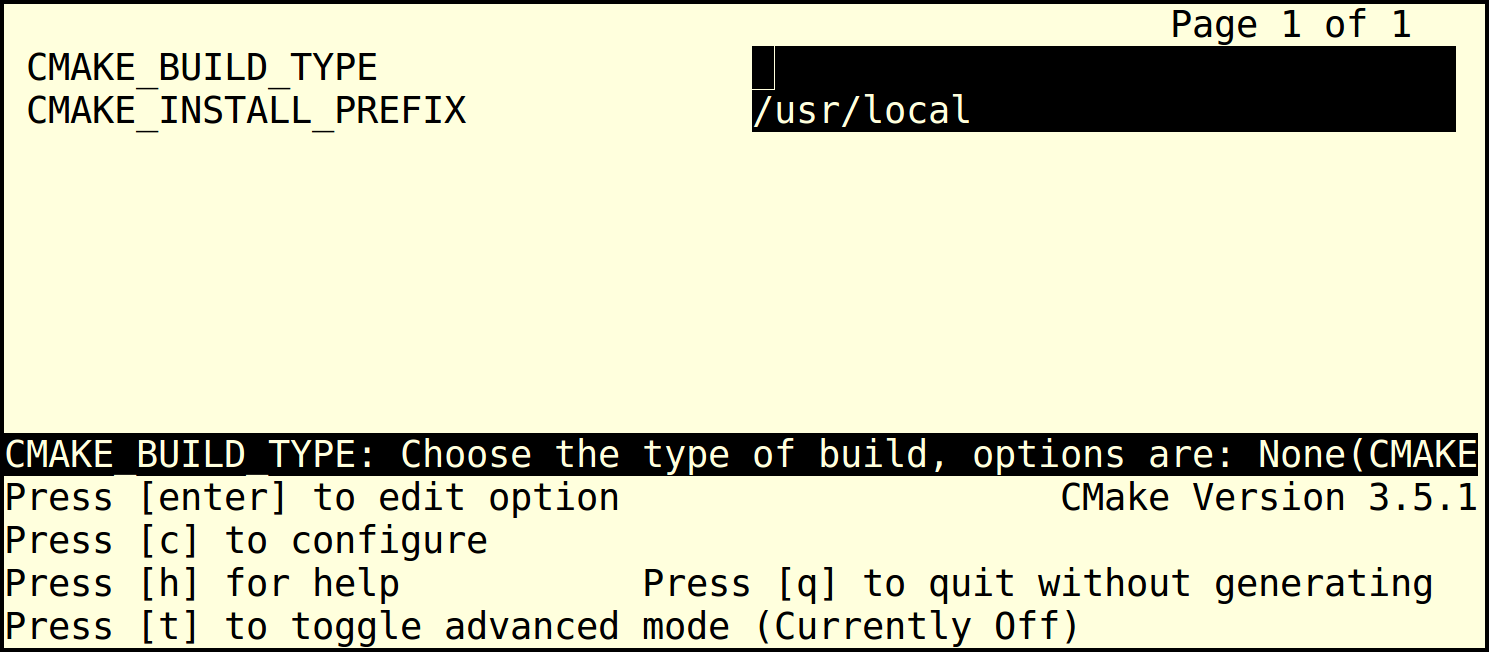
\includegraphics[height=0.4\textheight]{images/ccmake.png}
\end{frame}

\begin{frame}{Installazione}
  \texttt{CMakeLists.txt}
  \inputminted[bgcolor=codebackground,frame=single]{cmake}{examples/4-cmake-2/CMakeLists.txt}
\end{frame}

\begin{frame}{CMake: vantaggi}
  \begin{itemize}

  \item Funziona su Linux, Windows, MacOS\dots
  \item Diffusione crescente
  \item Apprendimento iniziale facile
  \item \texttt{ccmake} e \texttt{cmake-gui} per configurazione interattiva
  \item Genera \texttt{Makefile}, progetti Visual Studio, XCode\dots

  \item Vedi slide ``Cosa manca a Make'':
    \begin{itemize}
    \item Ricerca di librerie
    \item Prefix (\texttt{CMAKE\_INSTALL\_PREFIX})
    \item Diverted installation (\texttt{DESTDIR})
    \item Out of tree build
    \item Cross-compilazione
    \end{itemize}

  \end{itemize}
\end{frame}

\begin{frame}{CMake: svantaggi}
  \begin{itemize}
  \item Sintassi ``non convenzionale''
  \item Non è banale gestire software complessi in modo corretto
  \item Minore diffusione
  \end{itemize}
\end{frame}

\section{Conclusioni}

\begin{frame}{Conclusioni}
  \begin{itemize}
  \item Shell: non adatto
  \item Make: ottimo strumento, ma scrivere un ottimo
    \texttt{Makefile} è un lavoro enorme
  \item Autotools e CMake: strumenti completi e standard
    \begin{itemize}
    \item Fanno molto più di quanto abbiamo visto
    \item Esistono anche altri strumenti simili, meno diffusi
    \end{itemize}
  \end{itemize}
\end{frame}

\begin{frame}{Quale strumento utilizzare?}
  Priorità di scelta {\em indicativa}
  \begin{enumerate}
  \item {\bf Autotools o CMake}: quello che si conosce già
  \item {\bf CMake}:             se serve compilare su Windows, MacOS\dots
  \item {\bf Autotools}:         librerie di basso livello (sistema, interazione con il kernel)
  \item {\bf Make}:              se Autotools e CMake non sono adatti
  \item {\bf Shell}:             se non basta neanche Make\dots
  \end{enumerate}
\end{frame}

\begin{frame}{Bibliografia}
  \small
  \begin{itemize}
  \item GNU Make Manual (\url{https://www.gnu.org/software/make/manual/})
  \item ``A Practitioner's Guide to GNU Autoconf, Automake, and Libtool'',
    John Calcote (\url{https://www.nostarch.com/autotools.htm})
  \item ``Autotools Mythbuster'', Diego Elio “Flameeyes” Pettenò
    (\url{https://autotools.io/index.html})
  \item ``Autotools: A Demystification Tutorial'', Thomas Petazzoni
    (\url{https://elinux.org/images/4/43/Petazzoni.pdf},
    \url{https://www.youtube.com/watch?v=_zX8LJ9Xjyk})
  \item CMake Tutorial: \url{https://cmake.org/cmake-tutorial/}
  \item CMake documentation: \url{https://cmake.org/documentation/}
  \end{itemize}
\end{frame}

\begin{frame}
  \frametitle{Grazie per l'attenzione!}

  \begin{center}
    {\Huge Domande?}

    \vspace{0.1\textheight}

    \href{mailto:luca@lucaceresoli.net}{luca@lucaceresoli.net}\\
    \url{http://lucaceresoli.net}

    \textcopyright{} Copyright 2017, Luca Ceresoli\\

    \vspace{0.2\textheight}

    \tiny
    Materiale rilasciato sotto licenza\\
    Creative Commons Attribution - Share Alike 3.0 \\
    \url{https://creativecommons.org/licenses/by-sa/3.0/} \\
\end{center}
\end{frame}

\end{document}
